\documentclass[a4paper,12pt,fleqn]{article}
\usepackage[a4paper,margin=2cm]{geometry}
\usepackage{graphicx}
\usepackage{amsmath}
\usepackage{etoolbox}
\usepackage{caption}
\usepackage{algorithm}
\usepackage{algpseudocode}
\usepackage{float}
\usepackage{xcolor}
\usepackage{amssymb}
\usepackage[utf8]{inputenc}
\usepackage[T1]{fontenc}
\usepackage[french]{babel}
\usepackage[colorlinks=true, linkcolor=blue, citecolor=blue, urlcolor=blue]{hyperref}

\usepackage{tikz, pgfplots}
\usepackage{tikz-3dplot}
\pgfplotsset{compat=1.15}
\usetikzlibrary{calc}
\usetikzlibrary{arrows.meta}
\usetikzlibrary{intersections}
\usetikzlibrary{shapes}

%Nous définissons ici chacunes des figures, appelées comme des fonctions dans les autres documents.

\newcommand{\Grilleblank}{
    \draw[thick] (0,0) rectangle (5,7);
    \draw[step=1cm] (0,0) grid (5,7);
    \foreach \x in {0,...,4}
        \foreach \y in {0,...,6}
            \fill(\x+0.5, \y+0.5) circle(2pt);
    \fill(2.5, 3.5) circle(2pt) node[fill opacity=0, text opacity=1, above] {$\mathbf{C}$};
}

\newcommand{\distanceq}{
    \begin{tikzpicture}[baseline=(midpoint)]
    \coordinate (midpoint) at (0,1);
    \draw[step=1cm] (0,0) grid (2,2);
    \fill(0.5, 0.5) circle(2pt) node[below] at (0.5,0.58) {$P_{i,j+1}$};
    \fill(0.5, 1.5) circle(2pt) node[above] at (0.5,1.42) {$P_{i,j}$};
    \fill(1.5, 1.5) circle(2pt) node[above] at (1.5,1.42) {$P_{i+1,j}$};
    \fill(1.5, 1.5) circle(2pt);
    \draw[<->, red, thick] (0.5,0.5) -- (0.5,1.5);
    \draw[<->, red, thick] (0.5,1.5) -- (1.5,1.5);
    \end{tikzpicture}
}

\newcommand{\screenrepresentation}{
    \tdplotsetmaincoords{110}{55}
    \begin{tikzpicture}[scale=4, tdplot_main_coords]
    \tikzset{fortext/.style={
        fill=white, fill opacity=0.5, text opacity=1, rounded corners
    }}
    %axis
    \filldraw[red] (0,0,0) circle(1pt) node[anchor=north east] {$\mathbf{E}$};
    \draw[->, red, very thick] (0,0,0) -- (1,0,0) node[black, anchor=west] {$\mathbf{C}$};
    \draw[->, red, very thick] (0,0,0) -- (0,1,0) node[anchor=south] {$\vec{r}$};
    \draw[->, red, very thick] (0,0,0) -- (0,0,1) node[anchor=north east] {$\vec{u}$};
    %camera
    \coordinate (A) at (-0.8, -0.15, -0.15);
    \coordinate (B) at (-0.8, -0.15, 0.15);
    \coordinate (C) at (-0.8,  0.15, 0.15);
    \coordinate (D) at (-0.8,  0.15, -0.15);
    \coordinate (E) at (0, -0.15,  -0.15);
    \coordinate (F) at (0, -0.15,  0.15);
    \coordinate (G) at (0,  0.15,  0.15);
    \coordinate (H) at (0,  0.15, -0.15);

    \draw (A) -- (B) -- (C) -- (D) -- cycle;
    \draw (E) -- (F) -- (G) -- (H) -- cycle;
    \draw (A) node[below] {camera} -- (E);
    \draw (B) -- (F);
    \draw (C) -- (G);
    \draw (D) -- (H);

    %ray vectors
    \pgfmathsetmacro{\qx}{1/(3*sqrt(3))}; %la valeur de qx est egale a celle de qy ici
    \foreach \i in {1,...,7} {
        \foreach \j in {1,...,5} {
            \draw[gray, ->] (0,0,0) -- 
            (1,{(\j-1)*(\qx)-(2*\qx)},{(\i-1)*(\qx)-(3*\qx)});
            \draw[fill] (1,{(\j-1)*(\qx)-(2*\qx)},{(\i-1)*(\qx)-(3*\qx)}) circle [radius=0.4pt];
        }
    }

    %Grille
    \path (1,-{(5/2)*\qx},-{(7/2)*\qx}) coordinate (start);
    \foreach \i in {0,...,5} {
        \draw[thick] ($(start)+(0,{\i*\qx},0)$) -- ($(start)+(0,{\i*\qx},{(7*\qx)})$) ;
    }
    \foreach \i in {0,...,7} {
        \draw[thick] ($(start)+(0,0,{\i*\qx})$) -- ($(start)+(0,{(5*\qx)},{\i*\qx})$) ;
    }

    \end{tikzpicture}
}

\newcommand{\stretched}{
    \begin{tikzpicture}[scale=2]
        \draw (0,0) rectangle (2,2);
        \draw[<->, very thick] (0,-0.2) -- (2,-0.2) node[below, midway] {width};
        \draw[<->, very thick] (-0.2,0) -- (-0.2,2) node[left, midway] {height};
        \draw (0,1) -- (2,1);
        \draw (0.5,0) -- (0.5,2);
        \draw (1,0) -- (1,2);
        \draw (1.5,0) -- (1.5,2);
        \foreach \x in {0.25,0.75,1.25,1.75} {
            \draw[fill] (\x,0.5) circle (1pt);
            \draw[fill] (\x,1.5) circle (1pt);
        }
    \end{tikzpicture}
}

\newcommand{\unstretched}{
    \begin{tikzpicture}[scale=2]
        \draw (0,0) rectangle (4,2);
        \draw[<->, very thick] (0,-0.2) -- (4,-0.2) node[below, midway] {2$\times$width};
        \draw[<->, very thick] (-0.2,0) -- (-0.2,2) node[left, midway] {height};
        \draw (0,1) -- (4,1);
        \draw (1,0) -- (1,2);
        \draw (2,0) -- (2,2);
        \draw (3,0) -- (3,2);
        \foreach \x in {0.5,1.5,2.5,3.5} {
            \draw[fill] (\x,0.5) circle (1pt);
            \draw[fill] (\x,1.5) circle (1pt);
        }
    \end{tikzpicture}
}

\newcommand{\triangles}{
    \tdplotsetmaincoords{110}{55}
    \begin{tikzpicture}[scale=4, tdplot_main_coords]
    \tikzset{fortext/.style={
        fill=white, fill opacity=0.5, text opacity=1, rounded corners
    }}
    \pgfmathsetmacro{\qx}{1/(3*sqrt(3))};

    %camera
    \coordinate (A) at (-0.8, -0.15, -0.15);
    \coordinate (B) at (-0.8, -0.15, 0.15);
    \coordinate (C) at (-0.8,  0.15, 0.15);
    \coordinate (D) at (-0.8,  0.15, -0.15);
    \coordinate (E) at (0, -0.15,  -0.15);
    \coordinate (F) at (0, -0.15,  0.15);
    \coordinate (G) at (0,  0.15,  0.15);
    \coordinate (H) at (0,  0.15, -0.15);

    \draw (A) -- (B) -- (C) -- (D) -- cycle;
    \draw (E) -- (F) -- (G) -- (H) -- cycle;
    \draw (A) node[below, fortext] {camera} -- (E);
    \draw (B) -- (F);
    \draw (C) -- (G);
    \draw (D) -- (H);

    %Grille
    \draw[<->, very thick] ($(start)+(0,{5*\qx+0.05},0)$) -- ($(start)+(0,{5*\qx+0.05},{7*\qx})$) node[right, midway, fortext] {height};

    \path (1,-{(5/2)*\qx},-{(7/2)*\qx}) coordinate (start);
    \foreach \i in {0,...,5} {
        \draw[thick] ($(start)+(0,{\i*\qx},0)$) -- ($(start)+(0,{\i*\qx},{(7*\qx)})$) ;
    }
    \foreach \i in {0,...,7} {
        \draw[thick] ($(start)+(0,0,{\i*\qx})$) -- ($(start)+(0,{(5*\qx)},{\i*\qx})$) ;
    }

    %triangles
    \shadedraw[right color=orange!80!white, left color=gray, draw=orange!50!black, fill opacity=0.6] (0,0,0) -- (1,0,0) -- (1,0,{3.5*\qx}) -- cycle;
    \draw[<->, very thick, blue!80!black] (1,0,0) -- (1,0,{3.5*\qx}) node[right, midway, fortext] {$tan(\dfrac{\theta}{2})$};
    \shadedraw[right color=green!80!white, left color=gray, draw=green!50!black, fill opacity=0.6] (0,0,0) -- (1,0,0) -- (1,0,-{3.5*\qx}) -- cycle;
    \draw[<->, very thick, blue!80!white] (1,0,0) -- (1,0,-{3.5*\qx}) node[right, pos=0.3, fortext] {$tan(\dfrac{\theta}{2})$};

    %axis
    \filldraw[red] (0,0,0) circle(1pt) node[anchor=north east, fortext] {$\mathbf{E}$};
    \draw[->, red, very thick] (0,0,0) -- (1,0,0) node[black, anchor=west, fortext] {$\mathbf{C}$};
    \draw[->, red, very thick] (0,0,0) -- (0,1,0) node[anchor=south, fortext] {$\vec{r}$};
    \draw[->, red, very thick] (0,0,0) -- (0,0,1) node[anchor=north east, fortext] {$\vec{u}$};
    \draw[fill] (1,0,0) circle [radius=0.4pt];

    \end{tikzpicture}
}

\newcommand{\paritee}{
    \begin{tikzpicture}
    \node[right] at (-0.2,0.25) {Cas 1: w pair, h pair};
    \draw[step=1] (0,0) grid (4,-2);
    \foreach \x in {0.5,1.5,2.5,3.5} {
        \draw[fill] (\x,-0.5) circle (1pt);
        \draw[fill] (\x,-1.5) circle (1pt);
    }
    \draw[fill, purple] (2,-1) node[above] {$\mathbf{C}$} circle (1.5pt);
    \node[above] at (0.5,-0.6) {$P_{1,1}$};

    \begin{scope}[shift={(5.5,0)}]
        \node[right] at (-0.2,0.25) {Cas 2: w pair, h impair};
        \draw[step=1] (0,0) grid (4,-3);
        \foreach \x in {0.5,1.5,2.5,3.5} {
            \draw[fill] (\x,-0.5) circle (1pt);
            \draw[fill] (\x,-1.5) circle (1pt);
            \draw[fill] (\x,-2.5) circle (1pt);
        }
        \draw[fill, purple] (2,-1.5) node[above] {$\mathbf{C}$} circle (1.5pt);
        \node[above] at (0.5,-0.6) {$P_{1,1}$};
    \end{scope}

    \begin{scope}[shift={(0,-4.5)}]
        \node[right] at (-0.2,0.25) {Cas 3: w impair, h pair};
        \draw[step=1] (0,0) grid (3,-4);
        \foreach \x in {0.5,1.5,2.5} {
            \draw[fill] (\x,-0.5) circle (1pt);
            \draw[fill] (\x,-1.5) circle (1pt);
            \draw[fill] (\x,-2.5) circle (1pt);
            \draw[fill] (\x,-3.5) circle (1pt);
        }
        \draw[fill, purple] (1.5,-2) node[above] {$\mathbf{C}$} circle (1.5pt);
        \node[above] at (0.5,-0.6) {$P_{1,1}$};
    \end{scope}

    \begin{scope}[shift={(5.5,-4.5)}]
        \node[right] at (-0.2,0.25) {Cas 4: w impair, h impair};
        \draw[step=1] (0,0) grid (4,-4);
        \foreach \x in {0.5,1.5,2.5,3.5} {
            \draw[fill] (\x,-0.5) circle (1pt);
            \draw[fill] (\x,-1.5) circle (1pt);
            \draw[fill] (\x,-2.5) circle (1pt);
            \draw[fill] (\x,-3.5) circle (1pt);
        }
        \draw[fill, purple] (2,-2) node[above] {$\mathbf{C}$} circle (1.5pt);
        \node[above] at (0.5,-0.6) {$P_{1,1}$};
    \end{scope}
    \end{tikzpicture}
}
\setlength{\parindent}{0pt}
   
\begin{document}  
\sloppy

\begin{center}

\Huge
\begin{tabular}{l  l }
	\raisebox{-0.3\height}{ 
\includegraphics[scale=0.04]{include/upsaclay.png}} & \textbf{   Université Paris-Saclay} \\
	
\end{tabular}



\Huge
\vspace{2cm}
\textbf{Rapport PPN Semestre 1}


\vspace{1cm}
\Large
\textbf{Filière: M1 Calcul Haute Performance et Simulation}

\vspace{1cm}
Années: 2025-2026


\huge
\vspace{1.5cm}
\rule{\textwidth}{1pt}
\vspace{0.5cm}
\textbf{\underline{Sujet:} Path tracing: méthodes de \\
	Monte Carlo pour la synthèse d'images}
\rule{\textwidth}{1pt}

\vspace{2cm}

\begin{minipage}{.45\linewidth}
	
	\begin{flushleft}
		\large
		\textbf{Rédigé par:} \\
		Nolwen DOLLÉANS\\
		Prince Marcel MASSAMBA \\
		Théo BAUER \\
	\end{flushleft}
\end{minipage}
\hfill
\begin{minipage}{.45\linewidth}
	
	\begin{flushright}
		\large
		\textbf{Encadré par:} \\
		Mr. Aurélien DELVAL \\
		 
	\end{flushright}
\end{minipage}

\end{center}

\pagebreak
\tableofcontents
\pagebreak
\section{Définition de l'écran}

Nous définissons notre écran comme la formation d'une grille carré de pixels, la grille est de largeur $w$ (width) et de hauteur $h$ (height) en nombre de pixels. Chaque pixel a un centre qui intersecte la direction de chacun des rayons sortant de la caméra. Le centre de l'écran est le point $\mathbf{C} \in \mathbb{R}^3$ résultant de $\mathbf{E}+\vec{d}$, il se trouve ainsi à distance $1$ de la caméra. Nous définissons finalement un angle $\theta \in [-\pi,\pi]$ représetant la "Field Of View" (FOV).

Notons ici que l'écran forme un plan parrallèle à $(\vec{r},\vec{u})$ et qu'il dépend donc de l'orientation de la caméra.

Posons par exemple un écran formé par $7\times5$ pixels. La représentation finale dans $\mathbb{R}^3$ pour un FOV $\theta=\dfrac{\pi}{3}$ d'un tel écran est :

\screenrepresentation

\subsection{Aspect Ratio}
Or nous nous rendons compte que le nombre de pixels en width et en height ne sont pas toujours égaux, donc pour un même FOV nous obtenons un effet d'étirement de l'image. C'est pourquoi nous introduisons l'Aspect Ratio :

Nous pouvons visualiser un écran à  $(w,h)=(4,2)$ avant la prise en compte de l'aspect ratio :

\stretched

Les pixels ne sont pas carrés et lorsque nous représentont des objets sur ce type d'écran, nous voyons l'effet suivant :

\begin{figure}[H]
\centering
\begin{minipage}{.5\textwidth}
  \centering
  
\includegraphics[scale=0.2]{include/exemple480x480.png}
  \captionof{figure}{480x480 image}
  \label{fig:test1}
\end{minipage}%
\begin{minipage}{.5\textwidth}
  \centering
  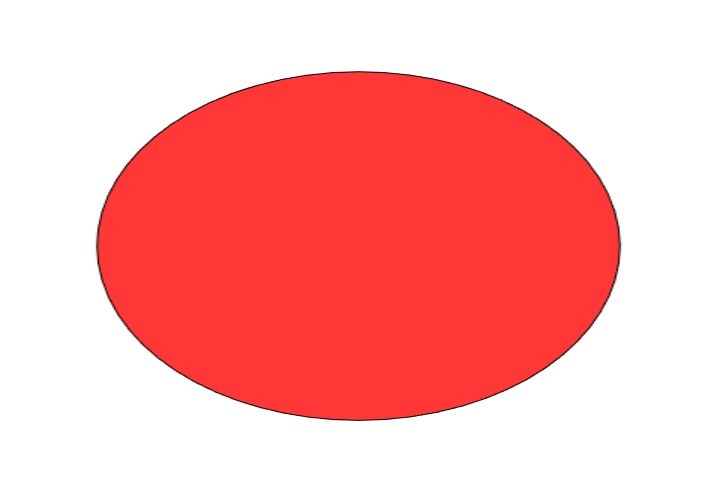
\includegraphics[scale=0.2]{include/exemple720x480.jpeg}
  \captionof{figure}{720x480 image}
  \label{fig:test2}
\end{minipage}
\begin{minipage}{.5\textwidth}
  \centering
  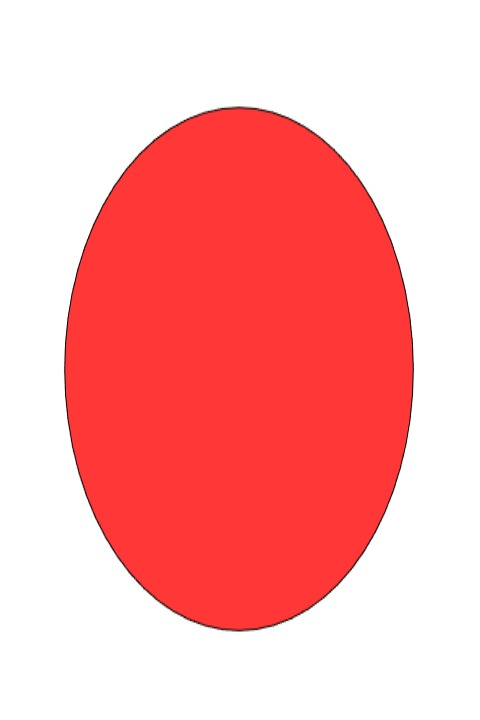
\includegraphics[scale=0.2]{include/exemple480x720.jpeg}
  \captionof{figure}{480x720 image}
  \label{fig:test3}
\end{minipage}
\end{figure}

L'aspect ratio se résume au quotient entre la width et la height de l'image en nombre de pixels : $AR=\dfrac{w}{h}$. Pour les figures ci-dessus : 

\begin{itemize}
    \item $AspectRatio_1 = \frac{480}{480} = 1$. \vspace{3pt}
    \item $AspectRatio_2 = \frac{720}{480} = 1.5 > 1$. \vspace{3pt}
    \item $AspectRatio_3 = \frac{480}{720} = 0.66 < 1$. \vspace{3pt}
\end{itemize}

Afin de corriger ce problème, nous multiplions la width $w$ par l'aspect ratio. Ainsi si $(w,h)=(4,2)$ :

$AspectRatio = \frac{4}{2} = 2$ \vspace{3pt}

\unstretched

\subsection{Obtention des vecteurs des rayons}
Nous voulons dans cette partie déterminer comment obtenir chacun des vecteurs dirigeant les rayons en fonction du nombre des pixels $(w,h)$ et de l'angle $\theta$.

Nous posons $\forall (i,j) \in \mathbb{N} \text{ tel que } 1\leq i\leq w, 1\leq j\leq h \; P_{i,j} \in \mathbb{R}^3$ chacun des centres des pixels tels que pour $(w,h)=(7,5)$ :

\begin{tikzpicture}
    \Grilleblank
    \node[above] at (0.5,6.41) {$P_{1,1}$};
    \node[above] at (4.5,6.41) {$P_{w,1}$};
    \node[below] at (0.5,0.59) {$P_{1,h}$};
    \node[below] at (4.5,0.59) {$P_{w,h}$};
\end{tikzpicture}

Par simples règles de trigonométrie sur des triangles rectangles, nous savons que :

\triangles

Remarquons que le résultat de cette distance sur la width est $\dfrac{w}{h}tan(\dfrac{\theta}{2})$, il suffit de multiplier par l'aspect ratio.

Nous pouvons maintenant chercher la distance séparant deux centres de pixels adjacents, c'est-à-dire la distance :

\distanceq et trouvons qu'elle est égale à $\dfrac{2\, tan(\dfrac{\theta}{2})}{w}$.

Nous savons que $\mathbf{C}=\mathbf{E}+\vec{d}=(0,0,1)$ et cherchons à déterminer les coordonnées de $P_{1,1}$ :

Avant cela, nous devons nous assurer de la position de $\mathbf{C}$ par rapport au centre des pixels sur l'écran. Celle-ci dépend de la paritée de $(w,h)$ donnant quatre cas de figure :

\paritee

Dans chacun de ces cas, nous pouvons tout de même obtenir les coordonnées de $P_{1,1}$ car aux vecteurs suivants : \\[0.5ex]
$\vec{d_{r}} = -2\, (\dfrac{w}{h})\, tan(\dfrac{\theta}{2}) \, \dfrac{w-1}{2w}\, \vec{r}$ \: et \: $\vec{d_{u}} = 2\, tan(\dfrac{\theta}{2}) \, \dfrac{h-1}{2h}\, \vec{u}$ \\[0.6ex]
Qui, partant de $\mathbf{C}$, pour $(w,h)=(5,7)$ sont visuellement représentées tels que : \\[0.6ex]
\begin{tikzpicture}
    \Grilleblank
    \node[above] at (0.5,6.41) {$P_{1,1}$};
    \draw[->, very thick, red] (2.5, 3.5) -- (0.5,3.5) node[below, midway, fill=white, fill opacity=0.5, text opacity=1, rounded corners] {$\vec{d_{r}}$};
    \draw[->, very thick, red] (2.5, 3.5) -- (2.5,6.5) node[right, midway, fill=white, fill opacity=0.5, text opacity=1, rounded corners] {$\vec{d_{u}}$};
\end{tikzpicture}

Nous en déduisons que les coordonnées de $P_{1,1}$ sont donc :

$P_{1,1}
=\vec{d_{r}}+\vec{d_{u}}+\mathbf{C}
=-tan(\dfrac{\theta}{2}) \, \dfrac{w-1}{h}\, \vec{r}+tan(\dfrac{\theta}{2}) \, \dfrac{h-1}{h}\, \vec{u}+\mathbf{C}$ \\[0.6ex]
$P_{1,1}
=\begin{pmatrix} -tan(\dfrac{\theta}{2}) \, \dfrac{w-1}{h}\\[1ex] 0\\0 \end{pmatrix}+\begin{pmatrix} 0\\ tan(\dfrac{\theta}{2}) \, \dfrac{h-1}{h}\\[1ex] 0 \end{pmatrix}+\begin{pmatrix} 0\\0\\1 \end{pmatrix}$ \\[0.6ex]
$P_{1,1}=\begin{pmatrix} -tan(\dfrac{\theta}{2}) \, \dfrac{w-1}{h}\\[1.3ex] tan(\dfrac{\theta}{2}) \, \dfrac{h-1}{h}\\[1.3ex] 1 \end{pmatrix}$.

De cette manière, nous pouvons finalement exprimer $P_{i,j}$ en fonction de $(w,h), \theta$ et $P_{1,1}$ :

$P_{i,j}=P_{1,1}+(i-1)\dfrac{2}{w}tan(\dfrac{\theta}{2})\vec{r}-(j-1)\dfrac{2}{h}tan(\dfrac{\theta}{2})\vec{u}$ \\[1.5ex]
$P_{i,j}=\begin{pmatrix} -tan(\dfrac{\theta}{2}) \, \dfrac{w-1}{h}\\[1.3ex] tan(\dfrac{\theta}{2}) \, \dfrac{h-1}{h}\\[1.3ex] 1 \end{pmatrix} + \begin{pmatrix} (i-1)\dfrac{2}{w}tan(\dfrac{\theta}{2})\vec{r}\\[1.3ex]0\\0 \end{pmatrix} + \begin{pmatrix} 0\\-(j-1)\dfrac{2}{h}tan(\dfrac{\theta}{2})\vec{u}\\[1.3ex]0 \end{pmatrix}$ \\[1.5ex]
$P_{i,j}=\begin{pmatrix} (i-1)\dfrac{2}{w}tan(\dfrac{\theta}{2})-tan(\dfrac{\theta}{2}) \, \dfrac{w-1}{h}\\[1.3ex] -(j-1)\dfrac{2}{h}tan(\dfrac{\theta}{2})+tan(\dfrac{\theta}{2}) \, \dfrac{h-1}{h}\\[1.3ex]1 \end{pmatrix}$ \\[2ex]
Et donc les vecteurs directeurs de chacun de ces points partant de la caméra sont :

$\forall (i,j) \in \mathbb{N} \text{ tel que } 1\leq i\leq w, 1\leq j\leq h, \; \vec{p_{i,j}} \in \mathbb{R}^3, \; \vec{p_{i,j}}=\overrightarrow{\mathbf{E}P_{i,j}}$ qui en particulier coïncide avec les coordonnées de $P_{i,j}$.

Nous voulons cependant normaliser ces vecteurs, nous définissons donc :

$\forall (i,j) \in \mathbb{N} \text{ tel que } 1\leq i\leq w, 1\leq j\leq h, \; \vec{r_{i,j}} \in \mathbb{R}^3, \; \vec{r_{i,j}}=\dfrac{\vec{p_{i,j}}}{\lVert \vec{p_{i,j}} \rVert}$. Les $\vec{r_{i,j}}$ sont les rayons normalisés sortant de la caméra dont nous connaissons maintenant les coordonnées.
\section{Définition d'objets dans l'espace}

\subsection{Équation d'un rayon}

Pour tout vecteur $\vec{d} \in \mathbb{R}^3$ d'origine $O \in \mathbb{R}^3$ dans la direction $T \in \mathbb{R}^3$, on a $\vec{d}=\overrightarrow{(O+T)}$ qui donne l'équation de rayon :

$$
\forall t  \in \mathbb{R}, \, 
{\vec{p}(t)} = {O + \vec{d}t} = \begin{pmatrix} o_x\\o_y\\o_z\end{pmatrix} + \begin{pmatrix} d_x\\d_y\\d_z\end{pmatrix}t =
\begin{pmatrix} o_x+d_xt\\o_y+d_yt\\o_z+d_zt\end{pmatrix}.
$$

\subsection{Équation d'une sphère}

Pour une position $C \in \mathbb{R}^3$ et un rayon $r \in \mathbb{R}_+$ on défini une sphère $s=(C, r)$ d'équation :

$$s = \{(x,y,z) \in \mathbb{R}^3 \, | \, (x - c_x)^2 + (y - c_y)^2 + (z - c_z)^2 = r^2 \}$$
$$\Leftrightarrow s = \{(x,y,z) \in \mathbb{R}^3 \, | \, (x - c_x)^2 + (y - c_y)^2 + (z - c_z)^2 - r^2 = 0 \}.$$

\subsection{Intersection d'un rayon sur une sphère}

Dans une premier temps, on injecte $\vec{p}(t)$ dans l'équation de $s(x,y,z)$, on obtient :

\begin{align*}
s(\vec{p}(t)) &= (p_x(t) - c_x)^2 + (p_y(t) - c_y)^2 + (p_z(t) - c_z)^2 - r^2 \\ 
              &= (o_x+d_x t - c_x)^2 + (o_y + d_y t - c_y)^2 + (o_z + d_z t- c_z)^2 - r^2 \\
              &= (d_x^2 + d_y^2 + d_z^2)t^2 + 2(o_x d_x + o_y d_y + o_z d_z - c_x d_x - c_y d_y - c_z d_z)t \\
              &\quad + (o_x^2 + o_y^2 + o_z^2 - c_x^2 - c_y^2 - c_z^2 - r^2) \\
              &= \lVert \vec{d} \rVert^2t^2 + 2\vec{d}\cdot(\overrightarrow{O-C})t + \lVert (\overrightarrow{O-C}) \rVert^2 - r^2
\end{align*}

Soit $s(\vec{p}(t))$ une équation quadratique, avec $a = \lVert \vec{d} \rVert^2$, $b = 2\vec{d}\cdot(\overrightarrow{O-C})$, $c = \lVert (\overrightarrow{O-C}) \rVert^2 - r^2$

On doit résoudre $at^2 + bt + c = 0$.

Pour un discriminant $\bigtriangleup = b^2 - 4ac$ : 

- Aucune intersection si $\bigtriangleup < 0$ ;

- Une intersection si $\bigtriangleup = 0 \Rightarrow x_1 = \dfrac{-b}{2a}$ ;

- Deux intersections si $\bigtriangleup > 0 \Rightarrow x_1 = \dfrac{-b - \sqrt{\bigtriangleup} }{2a}$, $x_2 = \dfrac{-b + \sqrt{\bigtriangleup} }{2a}$.

\begin{algorithm}
\caption{intersection Sphere}
\begin{algorithmic}
\Require Sphere, Ray and $hit \in \mathbb{R}^{3}$
\State $a = Ray.direction * Ray.direction$
\State $b = 2 * Ray.direction * (Ray.position - Ray.direction)$
\State $c = (Ray.position - Ray.direction)^2 - radius^2$

$\Delta = B^2 - 4AC$  

\If {$\Delta$ < 0}
   \State return $false$
\ElsIf {$\Delta == 0$}
    \State return $false$
\ElsIf {$\Delta > 0$}
    \State $t = \dfrac{-b}{2a}$
\ElsIf {$\Delta > 0$}
    \State $t = \dfrac{-b - \sqrt{\Delta}}{2a}$
\EndIf

\State $hit = Ray.position + Ray.direction * t$

\State return $true$

\end{algorithmic}
Complexité spatial : O(1)

Complexité temporel : O(1)
\end{algorithm}

\pagebreak
\section{AABB}

Un AABB (Axis-Aligned Bounding Box) est un pavé droit qui nous sert d'espace de rebond pour nos rayon.

Nous pouvons le définir par deux points $B_{min} \in \mathbb{R}^3, \, B_{max} \in \mathbb{R}^3$ représentant deux sommets aux extremitées du cube, chacunes des arêtes sont ensuite colinéaires à un des vecteurs de la base canonique.

\cubeblank

Nous traçons un rayon définit par $\vec{r}(t) = o + \vec{d}t$.

Dans le cas où il y a intersection :

\intersection

Nous avons 6 équations linéaire à résoudre :
$$
\begin{cases}
    xB_{\min} = o_{x} + d_{x}txB_{\min} \Longrightarrow txB_{\min} =  (xB_{\min} - o_{x})/d_{x} \\
    yB_{\min} = o_{y} + d_{y}tyB_{\min} \Longrightarrow tyB_{\min} =  (yB_{\min} - o_{y})/d_{y} \\
    zB_{\min} = o_{z} + d_{z}tzB_{\min} \Longrightarrow tzB_{\min} =  (zB_{\min} - o_{z})/d_{z} \\
    xB_{\max} = o_{x} + d_{x}txB_{\max} \Longrightarrow txB_{\max} =  (xB_{\max} - o_{x})/d_{x} \\
    yB_{\max} = o_{y} + d_{y}tyB_{\max} \Longrightarrow tyB_{\max} =  (yB_{\max} - o_{y})/d_{y} \\
    zB_{\max} = o_{z} + d_{z}tzB_{\max} \Longrightarrow tzB_{\max} =  (zB_{\max} - o_{z})/d_{z}
\end{cases}
$$

Ensuite, pour déterminer s'il y a intersection, on doit comparer la valeur maximale des solutions $tB_{i_\text{min}}$ à la valeur minimale des solutions $tB_{i_\text{max}}$:
\begin{itemize}
    \item $t_{\min} = max(txB_{\min}, tyB_{\min}, tzB_{\min})$
    \item $t_{\max} = min(txB_{\max}, tyB_{\max}, tzB_{\max})$
    \item Si il y a intersection, alors $t_{\min} < t_{\max}$
\end{itemize}

Dans le cas où il n'y a pas d'intersection :

\nointersection

Comme on peut le voir, $tyBmax < txBmin$ et $txBmax < tyBmin$, il ne peut pas y avoir une intersection.

\begin{algorithm}
\caption{intersection AABB}
\begin{algorithmic}

\Require AABB, Ray and $hit \in \mathbb{R}^{3}$
\State $tmin = \dfrac{bmin(0) - Ray.position(0)}{Ray.direction(0)}$
\State $tmax = \dfrac{bmax(0) - Ray.position(0)}{Ray.direction(0)}$

\If {$tmin > tmax$}
    \State swap($tmin$, $tmax$)
\EndIf

\For {i = 1 : 3}
    \State $t1 = \dfrac{bmin(i) - Ray.position(i)}{Ray.direction(i)}$
    \State $t2 = \dfrac{bmax(i) - Ray.position(i)}{Ray.direction(i)}$
    \If {$t1 > t2$}
        \State swap($tmin$, $tmax$)
    \EndIf
    \State $tmin = max(tmin, t1)$
    \State $tmax = min(tmax, t2)$

    \If {$tmin > tmax$}
        \State return $false$
    \EndIf
\EndFor

\State hit = Ray.position + Ray.direction * tmax

\State return $true$

\end{algorithmic}
Complexité spatial : O(1)\\
Complexité temporel : O(1)
\end{algorithm}

\pagebreak
\section{Équation de rendu}

L'équation de rendu représente l'impact de la radiance de la lumière sur une surface. En effet, elle va nous permettre de déterminer la manière dont la lumière se reflète sur un objet.

\begin{figure}[H]
	\bounce
	\centering 
	\captionof{figure}{Schéma de la réflection total des rayons de directions $\omega_i$ résultant en un rayon de direction $\omega_o$ sur le point $x$ d'une surface.}
\end{figure}

L'équation de rendu se définie comme suit (cf démonstration en Annexe 1):

$$\boxed{L_{o}(x, \omega_o) = L_{e}(x, \omega_o) + \int_{\Omega}f(x, \omega_o, \omega_i) \, L_{i}(x, \omega_i) \, \cos\left(\theta_i\right) \, d_{\omega_i}}$$

avec: 
\begin{itemize}
\item[$\_$] $\overrightarrow{n}$ : La normale de la surface au point $x$.
\item[$\_$] $\Omega$ : L'hémisphère centré autour de la normale $\textbf{n}$.
\item[$\_$] $x$ : Le point de $\mathbb{R}^3$ d'intersection entre les rayons incidents et la surface de l'objet considéré.
\item[$\_$] $\overrightarrow{\omega_o}$ : Direction du rayon réfléchis dans $\Omega$ sur la surface au point $x$.
\item[$\_$] $\overrightarrow{\omega_i}$ : Directions des rayons incidents dans $\Omega$ sur la surface au point $x$.
\item[$\_$] $L_o$ : La radiance réfléchis sur la surface au point $x$ de direction $\overrightarrow{\omega_o}$.
\item[$\_$] $L_e$ : La radiance émise par la surface au point $x$ de direction $\overrightarrow{\omega_o}$.
\item[$\_$] $L_i$ : Les radiances des rayons incidents sur la surface au point $x$ de direction $\overrightarrow{\omega_i}$.
\item[$\_$] $f$ : Le BRDF qui représente la manière dont le matériaux reflète la lumière.
\end{itemize}

\subsection{Les matériaux Lambertiens}

Cette équation n'est pas résoluble analytiquement. Pour faciliter les calculs et l'implémentation de notre path tracing, nous allons nous prendre le cas des matériaux dit "Lambertiens".\\

Ce type de matériaux inclus tous les matériaux de surface rugueuse qui n'émettent pas dans la lumière visible. Nous pouvons donc simplifier l'équation de rendu avec (cf démonstration Annexe 1):


$$ 
\boxed{L_o(x, \omega) = \frac\rho\pi \int_\Omega L_i(x, \omega_i) \, \cos\left(\theta_i\right) \, d_{\omega_i}}
$$

\subsection{Approximation avec la méthode Monte-Carlo}

La méthode de Monte-Carlo est une méthode itérative permettant de passer d'une intégrale à une somme d'échantillons aléatoires pondérée par une loi de probabilité notée $pdf$ (Probability Density Function). Cette somme converge vers la solution vraie en fonction du nombre d'échantillons.

Ainsi, nous avons l'approximation suivante:

Soit g, une fonction telle que: $g:\ \left\{
\begin{array}{l}
\mathbb{R} \longmapsto \mathbb{R}\\
x\longrightarrow g(x)
\end{array}
\right.$:
$$
I = \int_\Omega g(x) \, d_x \approx \frac{1}{N} \sum_k^N \frac{g(x_k)}{pdf(x_k)}
$$
\subsubsection{Méthode d'échantillonnage Cosine-Weighted} 

Pour des matériaux lambertiens, nous choisissons un échantillonnage dit "Cosine-weighted". Il consiste à se placer dans le repère local $(tangente, bitangente, normal)$ au point d'intersection (cf. \textit{Figure 9}), pour ensuite construire le rayon aléatoire.\\

\begin{figure}[H]
	\centering
\begin{minipage}{.4\textwidth}
	
	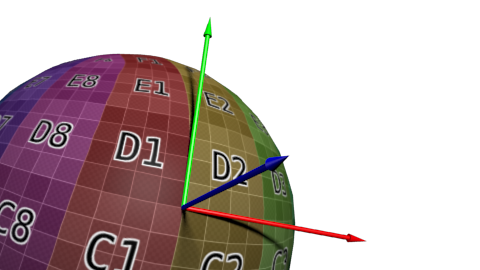
\includegraphics[scale=0.5]{include/NTBFromUVs.png}
\end{minipage}
\captionof{figure}{Représentation de la base locale au point d'intersection du rayon sur la sphère
avec la normale (en bleu), la bitangente (en vert) et la tangente (en rouge).}
\small{Source: https://www.opengl-tutorial.org/fr/intermediate-tutorials/tutorial-13-normal-mapping/}
\end{figure}

 Ce mode d'échantillonnage se fait de la manière suivante:
\begin{itemize}
\item[$\_$] Génération de 2 nombres aléatoires $\xi_1\in\mathbb{N}$ et $\xi_2\in\mathbb{N}$\\
\item[$\_$] On les passe en coordonnées polaires: $\left\{
\begin{array}{l}
r = \sqrt{\xi_1}\\
\theta = 2\pi\xi_2
\end{array}
\right.$
\item[$\_$] On passe les coordonnées polaires dans la base locale:$\left\{
\begin{array}{l}
x = r\cos\theta\\
y = r\sin\theta\\
z = \sqrt{1-r^2}
\end{array}
\right.$\\

\end{itemize} 
Ainsi, on construit la direction du rayon incident $\omega_i$ de la manière suivante dans la base $\left( right, up, forward\right)$: $\omega_i = x\cdot tangente + y\cdot bitangente+ z\cdot normal $.\\

L'avantage de cette méthode d'échantillonnage est que la $pdf$ sera: $pdf = \frac{\cos\theta_i}{\pi}$.

\subsubsection{Application de la Méthode de Monte-Carlo pour l'équation de rendu}

L'équation de rendu avec la méthode de Monte-Carlo s'écrit de la façon suivante:
\\
$$ 
L_o(x, \omega_o) = \frac\rho\pi \sum_{i=1}^N \frac{L_i(x, \omega_i) \, \cos\left(\theta_i\right)}{pdf(\omega_i)}
$$

$$ 
L_o(x, \omega_o) = \rho\sum_{i=1}^N {L_i(x, \omega_i)}
$$
\\

Ainsi, nous avons pu bien simplifier l'équation de rendu en choisissant le bon échantillonnage et en travaillant sur les bons matériaux.

\subsection{Implémentation}
Le choix que nous avons fait pour notre première version naïve est la suivante: la somme $\rho\sum_{i=1}^N {L_i(x, \omega_i)}$ est représentée dans notre code comme étant une fonction récursive. En effet, pour chaque rebond, nous allons sommer $\rho\ L_i(x, \omega_i)$ et retourner le résultat pour chaque échantillon de pixel. La fonction sera de la manière suivante:

\begin{algorithm}[H]
\caption{Échantillonnage récursif d’un rayon (RaySampling)}
\begin{algorithmic}[1]
\Require Rayon $r$, scène $S$, caméra $cam$, profondeur $d$, profondeur max $d_{\max}$
\Ensure Couleur incidente $L$
\State Initialiser $L \gets (0,0,0)$
\State $black \gets (0,0,0)$
\If{$d = d_{\max}$}
    \State \Return $black$
\EndIf
\If{pas d’intersection de $r$ avec la scène}
  \State \Return couleur de fond de la scène
\EndIf
\If{l’objet est émissif}
    \State $L \gets intensite \cdot couleur\_objet$
    \State \Return $L$
\EndIf
\State Générer un rayon réfléchi $r_{new}$ dans l’hémisphère selon une loi Cosine-Weighted

\State $L_{ref} \gets$ \Call{RaySampling}{$r_{new}, S, cam, d+1, d_{\max}$}
\State$L \gets L+albedo \cdot L_{ref}$
\State \Return $L$

\end{algorithmic}
\end{algorithm}



\pagebreak

\section{Demonstration sur les matrices de rotations}

Dans le cadre de ce projet, nous fixons la caméra à la position : $\mathbf{E} = (0, 0, 0)\in \mathbb{R}^3$ et nous posons être dans la base canonique de $\mathbb{R}^3$ : $(\vec{r_0}, \vec{u_0}, \vec{d_0}) =
\left(
\left( \begin{smallmatrix} 1 \\ 0 \\ 0 \end{smallmatrix} \right),
\left( \begin{smallmatrix} 0 \\ 1 \\ 0 \end{smallmatrix} \right),
\left( \begin{smallmatrix} 0 \\ 0 \\ 1 \end{smallmatrix} \right)
\right)$. Notons que jusqu'à maintenant la caméra pointe dans la direction de $\vec{d_0}$. En restant à cette position, nous allons implémenter la possibilité pour la caméra de pivoter dans n'importe quelle direction, nous cherchons donc ici à démontrer que l'application utilisée pour implémenter cela fonctionne pour n'importe quel angle choisi.

Pour réaliser cela, nous considérons un angle $\alpha$ présentant une rotation par rapport à l'axe formé par le vecteur $\vec{r_0}$ et un second angle $\beta$ présentant une rotation par rapport à l'axe formé par le vecteur $\vec{u_0}$.

L'application qui permet la rotation de la caméra est determinée par la composition des deux applications suivantes $\forall \alpha, \beta \in \mathbb{R}$ (nous pouvons restreindre $\alpha$ et $\beta$ à $[0, 2\pi]$ mais rien nous pose cette condition ici) :

$\begin{array}{ccccc}
pitch_\alpha & : & \mathbb{R}^3 & \to & \mathbb{R}^3 \\
 & & (x, y, z) & \mapsto & pitch_\alpha (x, y, z) \\
\end{array}
\quad$ et $\quad
\begin{array}{ccccc}
yaw_\beta & : & \mathbb{R}^3 & \to & \mathbb{R}^3 \\
 & & (x, y, z) & \mapsto & yaw_\beta (x, y, z) \\
\end{array}$

Qui sont toutes deux définies grâce aux matrices de rotations sur leurs axes respectifs :

\[ \forall \alpha \in \mathbb{R} : 
pitch_{\alpha}(x,y,z) = 
\begin{pmatrix}  0 & 0 & 1  \\ \sin\alpha & \cos\alpha & 0 \\ \cos\alpha & -\sin\alpha & 0 \end{pmatrix}
\begin{pmatrix} x \\ y \\ z \end{pmatrix}
= 
\begin{pmatrix} z \\ x\sin\alpha + y\cos\alpha  \\ x\cos\alpha - y\sin\alpha \end{pmatrix}
\]

\[ \forall \beta \in \mathbb{R} : 
yaw_{\beta}(x,y,z) = 
\begin{pmatrix} -\sin\beta & 0 & \cos\beta \\ 0 & 1 & 0 \\ \cos\beta & 0 & \sin\beta \end{pmatrix}
\begin{pmatrix} x \\ y \\ z \end{pmatrix}
= 
\begin{pmatrix} -x\sin\beta + z\cos\beta \\ y \\ x\cos\beta + z\sin\beta \end{pmatrix}
\]

Nous nous intérressons donc à l'application : $pitch_{\alpha} \circ yaw_{\beta}$ appliquée à chacun des vecteurs formant la base canonique. Soient les vecteurs $(\vec{r}, \vec{u}, \vec{d}) \in \mathbb{R}^3$ définis tels que $\forall \alpha, \beta \in \mathbb{R}$ : \\
$ \begin{cases}
pitch_{\alpha} \circ yaw_{\beta} \, (\vec{r_0}) = \vec{r} \\
pitch_{\alpha} \circ yaw_{\beta} \, (\vec{u_0}) = \vec{u} \\
pitch_{\alpha} \circ yaw_{\beta} \, (\vec{d_0}) = \vec{d} \\
\end{cases}$

Nous voulons montrer que la famille de vecteurs $(\vec{r}, \vec{u}, \vec{d})$ forment une base orthonormée de $\mathbb{R}^3$. C'est-à-dire qu'après utiliser cette application sur la position de la caméra, celle-ci pointerait maintenant dans la direction de $\vec{d}$. Soient $\alpha, \beta \in \mathbb{R}$.

Tout d'abord écrivons l'expression de $pitch_{\alpha} \circ yaw_{\beta} \; \forall (x, y, z) \in \mathbb{R}^3$ :

$pitch_{\alpha} \circ yaw_{\beta} \, (x, y, z) = \begin{pmatrix} x\cos\beta + z\sin\beta \\ (-x\sin\beta + z\cos\beta)\sin\alpha + y\cos\alpha \\ (-x\sin\beta + z\cos\beta)\cos\alpha - y\sin\alpha \end{pmatrix}$

Appliquons-la maintenant aux vecteurs de la base canonique : 

$\begin{cases}
\vec{r} = pitch_{\alpha} \circ yaw_{\beta} \, (\vec{r_0}) = \begin{pmatrix} \cos\beta \\ -\sin\alpha\sin\beta \\ -\cos\alpha\sin\beta \end{pmatrix}\\
\vec{u} = pitch_{\alpha} \circ yaw_{\beta} \, (\vec{u_0}) = \begin{pmatrix} 0 \\ \cos\alpha \\ -\sin\alpha \end{pmatrix} \\
\vec{d} = pitch_{\alpha} \circ yaw_{\beta} \, (\vec{d_0}) = \begin{pmatrix} \sin\beta \\ \cos\beta\sin\alpha \\ \cos\alpha\cos\beta \end{pmatrix} \\
\end{cases}$

Montrons premièrement que chacun de ces vecteurs sont de norme $1$ :
\begin{align*}
\| \vec{r} \|^2 &= \cos^2\beta+\sin^2\alpha\sin^2\beta+\cos^2\alpha\sin^2\beta \\
                &= \cos^2\beta+sin^2\beta(\sin^2\alpha+\cos^2\alpha) \\
                &= \cos^2\beta+sin^2\beta \\
                &= 1 \\[2mm]
\| \vec{u} \|^2 &= \cos^2\alpha+\sin^2\alpha \\
                &= 1 \\[2mm]
\| \vec{d} \|^2 &= \sin^2\beta+\cos^2\beta\sin^2\alpha+\cos^2\alpha\cos^2\beta \\
                &= \sin^2\beta+\cos^2\beta(\sin^2\alpha+\cos^2\alpha) \\
                &= \sin^2\beta+\cos^2\beta \\
                &= 1 \\[2mm]
\end{align*}
Calculons maintenant le produit vectoriel de $\vec{r}$ avec $\vec{u}$ :
\begin{align*}
\vec{r} \wedge \vec{u} &= \begin{pmatrix} \sin^2\alpha\sin\beta+\cos^2\alpha\sin\beta \\ \cos\beta\sin\alpha \\ \cos\alpha\cos\beta \end{pmatrix} \\
                       &= \begin{pmatrix} \sin\beta(\sin^2\alpha+\cos^2\alpha) \\ \cos\beta\sin\alpha \\  \cos\alpha\cos\beta \end{pmatrix} \\
                       &= \begin{pmatrix} \sin\beta \\ \cos\beta\sin\alpha \\ \cos\alpha\cos\beta \end{pmatrix} \\
                       &= \vec{d}
\end{align*}
Nous remarquons que le vecteur $\vec{d}$ est normal au plan formé par $\vec{r}$ et $\vec{u}$. Il nous reste donc à montrer que $\vec{r}$ et $\vec{u}$ sont orthogonaux :
\begin{align*}
\langle \vec{r}, \vec{u} \rangle &= \cos\beta\times0-\sin\alpha\sin\beta\cos\alpha+\cos\alpha\sin\beta\sin\alpha \\
                                 &= 0
\end{align*}
Nous avons montré que $\vec{d}$ est normal à $\vec{r}$ et $\vec{u}$; que $\vec{r}$ et $\vec{u}$ sont orthogonaux entre eux et que les trois vecteurs ont pour norme $1$. Cela montre donc que $(\vec{r},\vec{u}, \vec{d})$ est une base orthonormée de $\mathbb{R}^3$, donc que l'application $pitch_{\alpha} \circ yaw_{\beta}$ établi une rotation de la base canonique $(\vec{r_0}, \vec{u_0}, \vec{d_0})$ pour des $\alpha, \beta \in \mathbb{R}$ quelconques. Donc cette application nous permet bien de pivoter la caméra dans n'importe quelle direction, c'est-à-dire en considérant la sphère centrée en $\mathbf{E}$ de rayon $\| \vec{d_0} \| = 1 $ incluse dans $\mathbb{R}^3$ :

$\forall x \in (\mathbf{E}, \| \vec{d_0} \|), \exists \alpha, \beta \in \mathbb{R} \, \, \text{tels que} \, pitch_{\alpha} \circ yaw_{\beta}(\vec{d_0}) = \vec{\mathbf{E}x} $. 

\pagebreak


\end{document}